\chapter{Benchmark Components}\label{ch:appendix}
This appendix provides supplementary reference material for the benchmark introduced in Chapters \ref{ch:methodology} and \ref{ch:implementation}. Section \ref{sec:metrics-description} documents every metric used for evaluation and reward calculation in detail, building on the category-level overview of Section \ref{ssec:metric-categories} and the reward function of Section \ref{sec:agent-integration}. Section \ref{sec:result-visuals} then provides further examples of the result formats introduced in Section \ref{sec:result-format}.


\section{Metrics}\label{sec:metrics-description}
This section lists all metrics available in \benchmark. Section \ref{ssec:bench-metrics-description} documents the metrics used for agent evaluation, using the categories introduced in Section \ref{ssec:metric-categories}, while Section \ref{ssec:reward-metrics-description} documents the metrics available for the configurable reward function defined in Section \ref{sec:agent-integration}.


\subsection{Benchmark Metrics}\label{ssec:bench-metrics-description}
Table \ref{tab:metric_categories} lists all the metrics that \benchmark uses to evaluate agents. It is split into five sections, after the categories introduced in Section \ref{ssec:metric-categories}, and lists all the metrics in each category. For each metric the worst and best value is documented, which is used to map the metric into a normalised score from 0 to 100 as shown in Section \ref{ssec:score-calc}. Each metric is described in detail in the following subsections.

\begin{table}[htbp]
\centering
\footnotesize
\caption{Overview of metric categories, corresponding metrics, and scoring bounds}
\label{tab:metric_categories}
\begin{tabular}{ | p{0.17\textwidth} | p{0.43\textwidth} | p{0.17\textwidth} | p{0.13\textwidth} |}
\hline
\textbf{Category} & \textbf{Metric} & \textbf{Worst value} & \textbf{Best value} \\
\hline

\multirow{7}{=}{Overload mitigation}
& Timesteps without overload & 0 & $ep_{len}$ \\
& Total lines overloaded & $lines_{len} \cdot ep_{len}$  & 0 \\
& Max line loading timestep $N-0$ & 100 & 0 \\
& Mean line loading timestep $N-0$ & 100 & 0 \\
& Total lines overloaded timestep $N-0$ & $lines_{len}$ & 0 \\
& Max line loading $N-1$ & 100 & 0 \\
& Total lines overloaded timestep $N-1$ & $lines_{len}$ & 0 \\
\hline

\multirow{4}{=}{Voltage violation mitigation}
& Total timesteps with voltage violation & $ep_{len}$  & 0 \\
& Max voltage timestep deviation & 0.05 & 0 \\
& Mean voltage timestep deviation & 0.05 & 0 \\
& Percent bus voltage violation & 100 & 0 \\
\hline

\multirow{1}{=}{Survival}
& Survived iterations & 0 & $ep_{len}$ \\
\hline

\multirow{5}{=}{Costs}
& Timesteps without actions & 0 & $ep_{len}$ \\
& Substation changes & $ep_{len}$ & 0 \\
& Active power loss timestep percent & 100 & 0 \\
& Timesteps with load shedding & $ep_{len}$ & 0 \\
& Load shedding timestep percent & 100 & 0 \\
\hline

\multirow{3}{=}{Computational performance}
& Runtime timestep & $2 * val_{dn}$ & $val_{dn}$ \\
& CPU usage timestep & $2* val_{dn}$ & $val_{dn}$ \\
& Memory usage timestep & $2* val_{dn}$ & $val_{dn}$ \\
\hline

\end{tabular}
\end{table}

\FloatBarrier

\subsubsection{Overload Mitigation}
\label{app:metrics_overload_mitigation}

\textbf{Timesteps without overload:} The number of timesteps in the episode during which no transmission line exceeds 100\% of its rated loading. The best value is the full episode length $ep_{len}$, since every timestep was without overloads. The worst value is 0, meaning every timestep had at least one overloaded line.

\textbf{Total lines overloaded:} The cumulative number of overloaded lines summed across all timesteps of the episode. For each timestep, the number of lines exceeding 100\% loading is added to a running total. The best value is 0, meaning no line was ever overloaded. The worst value is $lines_{len} \cdot ep_{len}$, meaning every line was overloaded in every timestep.

\textbf{Max line loading timestep $N-0$:} For each timestep, the highest line loading percentage among all transmission lines in $N-0$ is recorded. This per-timestep maximum is aggregated across the episode using both the mean and the worst (highest) value. The best value is 0\%, the worst value is 100\%.

\textbf{Mean line loading timestep $N-0$:} For each timestep, the average line loading percentage across all transmission lines in the base case is calculated. This per-timestep average is aggregated across the episode using both the mean and worst value. The best value is 0\%, the worst value is 100\%.

\textbf{Total lines overloaded timestep $N-0$:} For each timestep, the number of lines exceeding 100\% loading in the base case is counted. This per-timestep count is aggregated across the episode using both the mean and worst value. The best value is 0, the worst value is $lines_{len}$.

\textbf{Max line loading $N-1$:} Using $N-1$ contingency analysis, each transmission line is temporarily removed one at a time, and the resulting maximum line loading among the remaining lines is calculated for every contingency. The highest of these values per timestep is recorded and aggregated across the episode using the mean and worst value. This metric indicates how close the grid is to a critical state should any single line fail. The best value is 0\%, the worst value is 100\%.

\textbf{Total lines overloaded timestep $N-1$:} Analogous to the $N-0$ version, but computed under $N-1$ contingency analysis. For each simulated single-line failure, the number of resulting overloaded lines is counted, and the highest count across all contingencies for that timestep is recorded. This per-timestep value is aggregated across the episode using the mean and worst value. The best value is 0, the worst value is $lines_{len}$.


\subsubsection{Voltage Violation Mitigation}
\label{app:metrics_voltage_violation_mitigation}

\textbf{Total timesteps with voltage violation:} The number of timesteps during which at least one bus voltage lies outside the permissible operating range of more than 5\% of its nominal value. The best value is 0, the worst value is $ep_{len}$.

\textbf{Max voltage timestep deviation:} For each timestep, the largest absolute deviation of any bus voltage from its nominal value is recorded. This per-timestep maximum is aggregated across the episode using the mean and worst value. The best value is 0, the worst value is 0.05 (representing a 5\% deviation; larger deviations are clipped).

\textbf{Mean voltage timestep deviation:} For each timestep, the average absolute deviation of all bus voltages from their nominal value is calculated. This per-timestep average is aggregated across the episode using the mean and worst value. The best value is 0, the worst value is 0.05.

\textbf{Percent bus voltage violation:} For each timestep, the percentage of buses whose voltage lies outside the permissible range is calculated. This per-timestep percentage is aggregated across the episode using the mean and worst value. The best value is 0\%, the worst value is 100\%.


\subsubsection{Survival}
\label{app:metrics_survival}

\textbf{Survived iterations:} The number of timesteps the agent kept the power grid in a stable, converged state before the episode ended or the simulation terminated due to non-convergence. The best value is $ep_{len}$, the worst value is 0.


\subsubsection{Costs}
\label{app:metrics_costs}

\textbf{Timesteps without actions:} The number of timesteps during which the agent chooses not to act on the grid at all. The best value is $ep_{len}$, the worst value is 0.

\textbf{Substation changes:} The amount of actions of the agent, that caused substation changes. The best value is 0 (no substation changes), the worst is $ep_{len}$ (every timestep of the episode one substation change).

\textbf{Active power loss timestep percent:} For each timestep, the active power lost in transmission lines and transformers (see Equation \eqref{eq:heat_power_dc}) is summed and expressed as a percentage of the total active power consumed by all loads in that timestep. If no load is present, this metric is defined as 0\%. This per-timestep percentage is aggregated across the episode using the mean and worst value. The best value is 0\%, the worst value is 100\%.

\textbf{Timesteps with load shedding:} The number of timesteps during which at least one load receives insufficient or no electricity. The best value is 0, the worst value is $ep_{len}$.

\textbf{Load shedding timestep percent:} For each timestep, the percentage of total demanded load that could not be supplied is calculated. This per-timestep percentage is aggregated across the episode using the mean and worst value. The best value is 0\%, the worst value is 100\%.


\subsubsection{Computational Performance}
\label{app:metrics_computational_performance}

\textbf{Runtime timestep:} The time required to compute a single timestep, i.e. one agent action and the resulting power flow calculation, measured in seconds. This is aggregated across the episode using the mean and worst (slowest) value. The best value is $val_{dn}$, the runtime of the do-nothing agent on the same scenario. The worst value is $2 \cdot val_{dn}$, twice this reference runtime.

\textbf{CPU usage timestep:} The CPU utilisation in percent measured while processing a single timestep, aggregated across the episode using the mean and worst value. The best value is $val_{dn}$, which is the CPU usage of the do-nothing agent on the same scenario, the worst value is $2 \cdot val_{dn}$.

\textbf{Memory usage timestep:} The memory consumption in percent measured while processing a single timestep, aggregated across the episode using the mean and worst value. The best value is $val_{dn}$, as the memory usage of the do-nothing agent on the same scenario, the worst value is $2 \cdot val_{dn}$.




\subsection{Reward Metrics}\label{ssec:reward-metrics-description}
Table \ref{tab:reward_metrics} lists all the metrics that are available for the configurable reward function presented in Section \ref{sec:agent-integration}. Each metric is grouped after categories and contains information about the worst and best value, which  is used to normalise the metric into a score in $[0,1]$. Each metric is described in detail in the following subsections.

\begin{table}[htbp]
\centering
\small
\caption{Overview of reward metrics and their scoring bounds}
\label{tab:reward_metrics}
\begin{tabular}{ | p{0.22\textwidth} | p{0.38\textwidth} | p{0.15\textwidth} | p{0.15\textwidth} |}
\hline
\textbf{Category} & \textbf{Metric} & \textbf{Worst value} & \textbf{Best value} \\
\hline

\multirow{3}{=}{Overloads}
& Max line loading $N-0$ & 100 & 0 \\
& Mean line loading $N-0$ & 100 & 0 \\
& Lines overloaded $N-0$ & $lines_{len}$ & 0 \\
\hline

\multirow{3}{=}{Voltage Violation}
& Max voltage deviation & 0.05 & 0 \\
& Mean voltage deviation & 0.05 & 0 \\
& Percent bus voltage violation & 100 & 0 \\
\hline

\multirow{2}{=}{Costs}
& Active power loss percent & 100 & 0 \\
& Load shedding percent & 100 & 0 \\
\hline

\end{tabular}
\end{table}

\FloatBarrier

\subsubsection{Overload}

\textbf{Max line loading $N-0$:} The highest line loading percentage among all transmission lines in $N-0$ for the current timestep. The best value is 0\%, the worst value is 100\%.

\textbf{Mean line loading $N-0$:} The average line loading percentage across all transmission lines in $N-0$ for the current timestep. The best value is 0\%, the worst value is 100\%.

\textbf{Lines overloaded $N-0$:} The number of transmission lines exceeding 100\% loading in the current timestep, in the base case. The best value is 0, the worst value is $lines_{len}$, the total number of lines in the network.

\subsubsection{Voltage Violation}

\textbf{Max voltage deviation:} The largest absolute deviation of any bus voltage from its nominal value in the current timestep. The best value is 0, the worst value is a deviation of 5\%.

\textbf{Mean voltage deviation:} The average absolute deviation of all bus voltages from their nominal value in the current timestep. The best value is 0, the worst value is a deviation of 5\%.

\textbf{Percent bus voltage violation:} The percentage of buses whose voltage lies outside of $\pm5\%$ of the nominal value in the current timestep. The best value is 0\%, the worst value is 100\%.

\subsubsection{Costs}

\textbf{Active power loss percent:} The active power lost in transmission lines and two-winding transformers in the current timestep, expressed as a percentage of the total active power served to all loads. If no load is served, this metric is defined as 0\%. The best value is 0\%, the worst value is 10\%.

\textbf{Load shedding percent:} The unserved active power in the current timestep, expressed as a percentage of the total requested active power from all in-service loads. Requested load is calculated from each load's rated power and scaling factor, while served load is taken from the power flow results. If no load is requested, this metric is defined as 0\%. The best value is 0\%, the worst value is 100\%.




\section{Result Visualisation Examples}\label{sec:result-visuals}
This section provides examples for the visualisation of benchmark results, introduced in Section \ref{sec:result-format}. Unless stated otherwise, all examples were generated by evaluating the do-nothing baseline agent introduced in Section \ref{sec:agent-integration}.


\subsection{Experiment Plots}\label{ssec:experiment-plots}
Figure \ref{fig:eval-plots} shows the five overview plots generated across all scenarios of an experiment, explained in Section \ref{ssec:visual-feedback}.

\begin{figure}[htp]
    \centering
    % Row 1
    \begin{subfigure}[t]{0.7\textwidth}
        \centering
        
\includegraphics[width=\textwidth]{images/appendix/example_plots/DN_category_heatmap.png}
        \caption{Heatmap showing category score for each scenario}
        \label{fig:eval-heatmap}
    \end{subfigure}

    \vspace{0.5em}

    % Row 2
    \begin{subfigure}[t]{0.49\textwidth}
        \centering
        
\includegraphics[width=\textwidth]{images/appendix/example_plots/DN_score_distribution.png}
        \caption{Score distribution over each scenario}
        \label{fig:eval-score-dist}
    \end{subfigure}
    \hfill
    \begin{subfigure}[t]{0.49\textwidth}
        \centering
        
\includegraphics[width=\textwidth]{images/appendix/example_plots/DN_category_score_distribution.png}
        \caption{Score distribution over categories}
        \label{fig:eval-category-score-dist}
    \end{subfigure}

    \caption{Overview of generated evaluation plots}
    \label{fig:eval-plots}
\end{figure}

\begin{figure}[htp]
    \ContinuedFloat
    \centering
    % Row 3
    \begin{subfigure}[t]{0.49\textwidth}
        \centering
        
\includegraphics[width=\textwidth]{images/appendix/example_plots/DN_scenario_comparison.png}
        \caption{Comparison of scenario scores}
        \label{fig:eval-scenario-comparison}
    \end{subfigure}
    \hfill
    \begin{subfigure}[t]{0.49\textwidth}
        \centering
        
\includegraphics[width=\textwidth]{images/appendix/example_plots/DN_score_progression.png}
        \caption{Comparison of run scores}
        \label{fig:eval-score-progression}
    \end{subfigure}

    \caption{Overview of generated evaluation plots (continued)}
\end{figure}

\FloatBarrier

\newpage
\subsection{Scenario Plots}\label{app:scenario-plots}
Figure \ref{fig:eval-scenario-plots} shows the three scenario-level plots generated for each individual scenario, explained in Section \ref{ssec:visual-feedback}.

\begin{figure}[htp]
    \centering
    % Row 1
    \begin{subfigure}[t]{0.6\textwidth}
        \centering
        
\includegraphics[width=\textwidth]{images/appendix/example_plots/category_radar.png}
        \caption{Radar graph showing average category scores}
        \label{fig:eval-radar}
    \end{subfigure}

    \vspace{0.5em}

    % Row 2
    \begin{subfigure}[t]{0.49\textwidth}
        \centering
        
\includegraphics[width=\textwidth]{images/appendix/example_plots/category_scores_bar.png}
        \caption{Category scores for each run}
        \label{fig:eval-category-bar}
    \end{subfigure}
    \hfill
    \begin{subfigure}[t]{0.49\textwidth}
        \centering
        
\includegraphics[width=\textwidth]{images/appendix/example_plots/score_over_index.png}
        \caption{Run scores over index}
        \label{fig:eval-score-index}
    \end{subfigure}

    \caption{Overview of generated evaluation plots}
    \label{fig:eval-scenario-plots}
\end{figure}

\FloatBarrier

\subsection{Summary Web Application}\label{app:webapp}
Figure \ref{fig:webapp-screenshots} shows screenshots of the Streamlit-based summary web application, which is introduced in Section \ref{ssec:visual-feedback}.

\begin{figure}[htp]
    \centering
    \begin{subfigure}[t]{\textwidth}
        \centering
        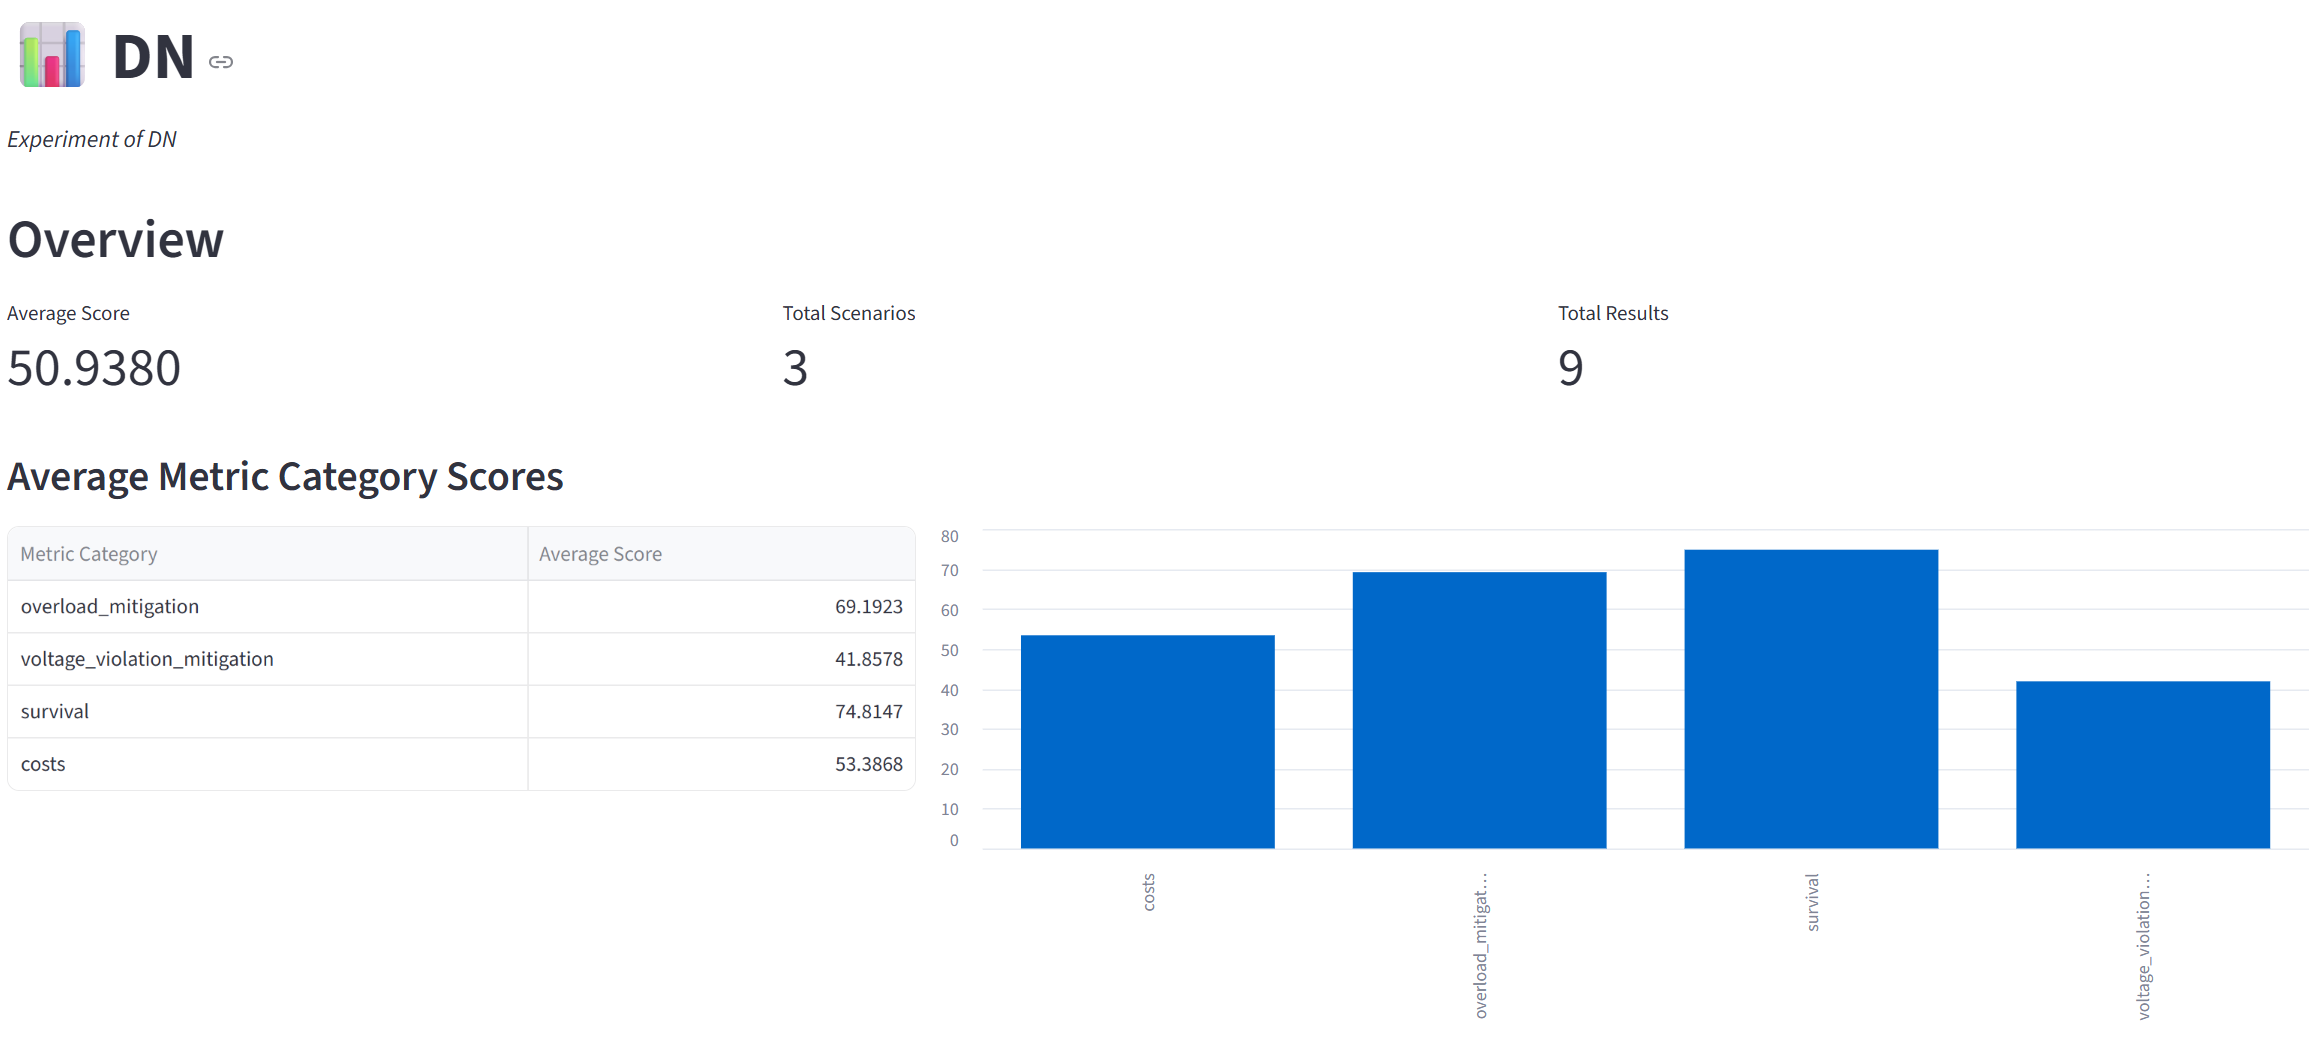
\includegraphics[width=\textwidth]{images/appendix/webapp/webapp_overview.png}
        \caption{Overview section}
        \label{fig:webapp-overview}
    \end{subfigure}

    \vspace{0.1em}

    \begin{subfigure}[t]{\textwidth}
        \centering
        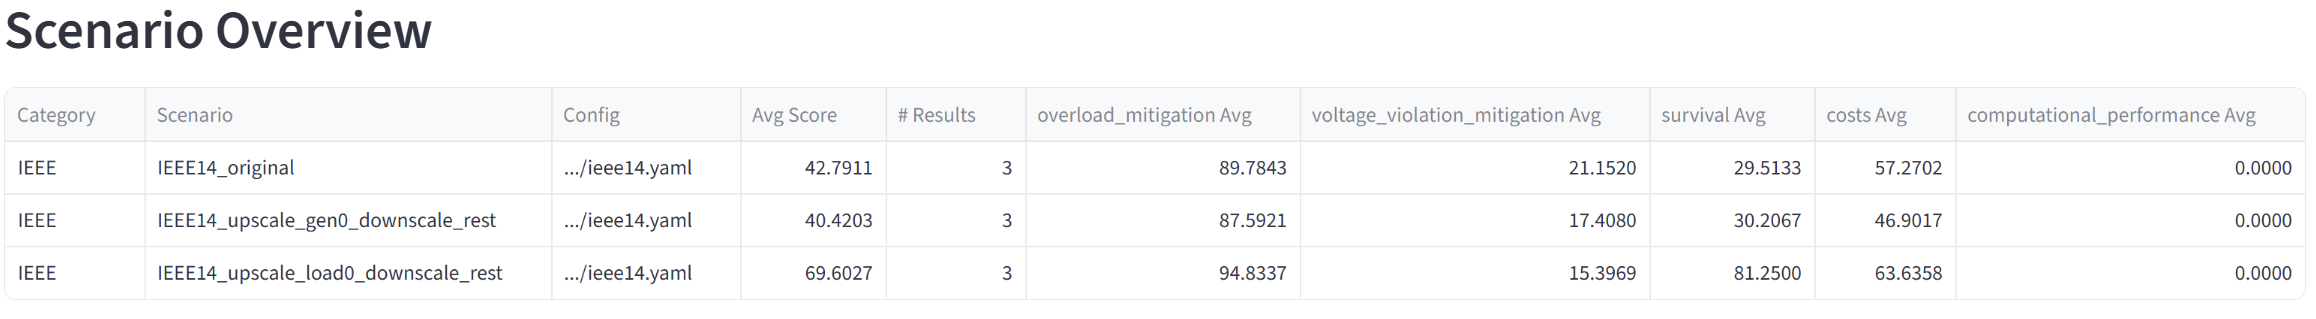
\includegraphics[width=\textwidth]{images/appendix/webapp/webapp_scenario_overview.png}
        \caption{Scenario overview section}
        \label{fig:webapp-scenario-overview}
    \end{subfigure}

    \vspace{0.1em}
    
    \begin{subfigure}[t]{\textwidth}
        \centering
        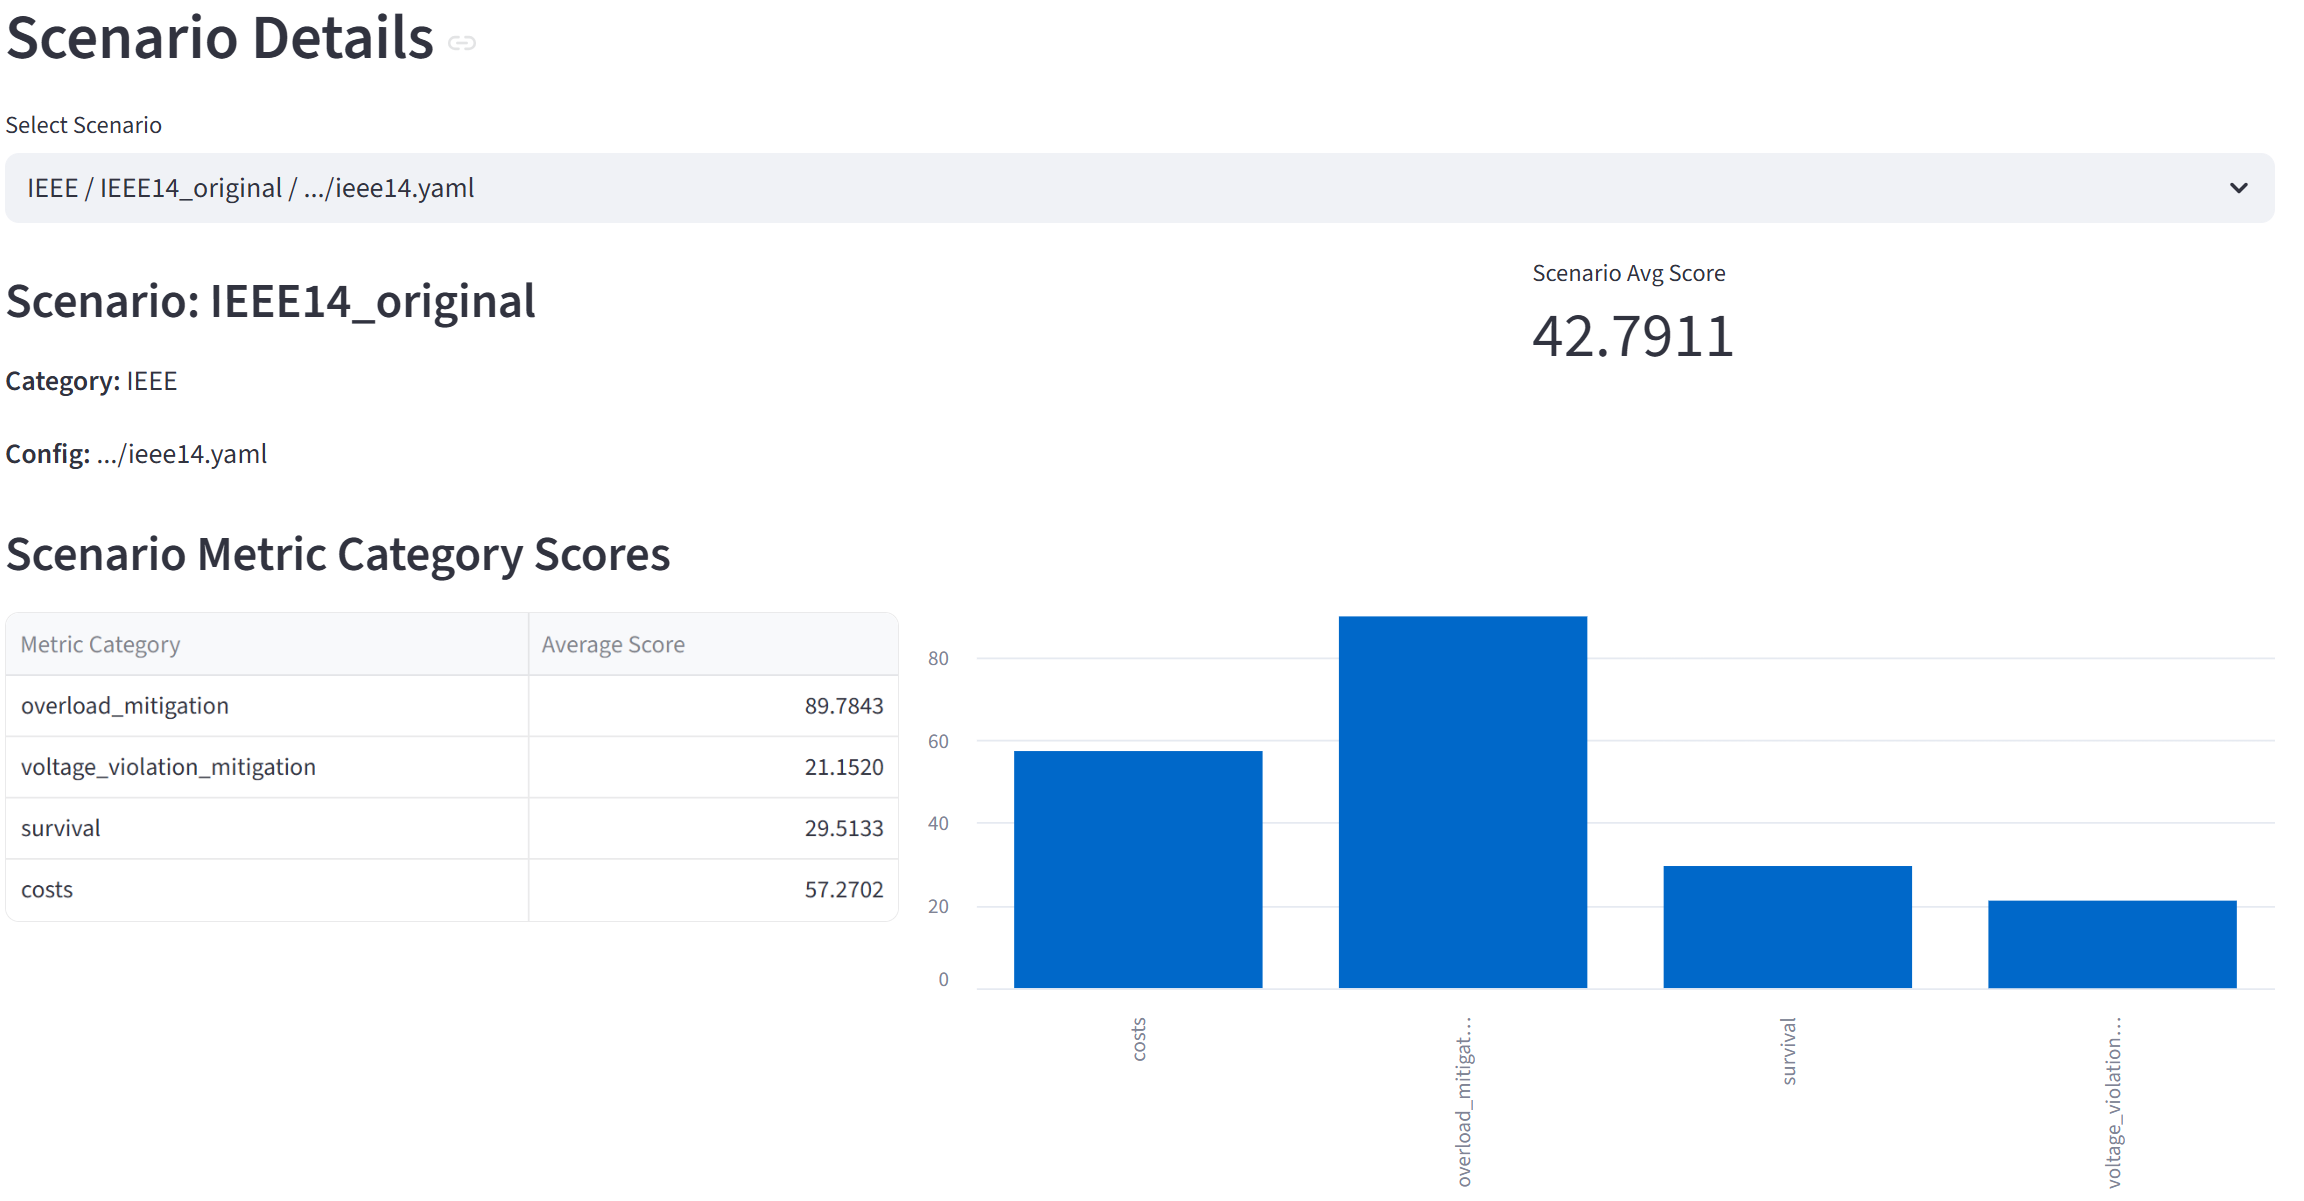
\includegraphics[width=\textwidth]{images/appendix/webapp/webapp_scenario_details.png}
        \caption{Scenario details section}
        \label{fig:webapp-scenario-details}
    \end{subfigure}

    \caption{Overview over webapp sections}
    \label{fig:webapp-screenshots}
\end{figure}

\begin{figure}[htp]
    \ContinuedFloat
    \centering

    \begin{subfigure}[t]{\textwidth}
        \centering
        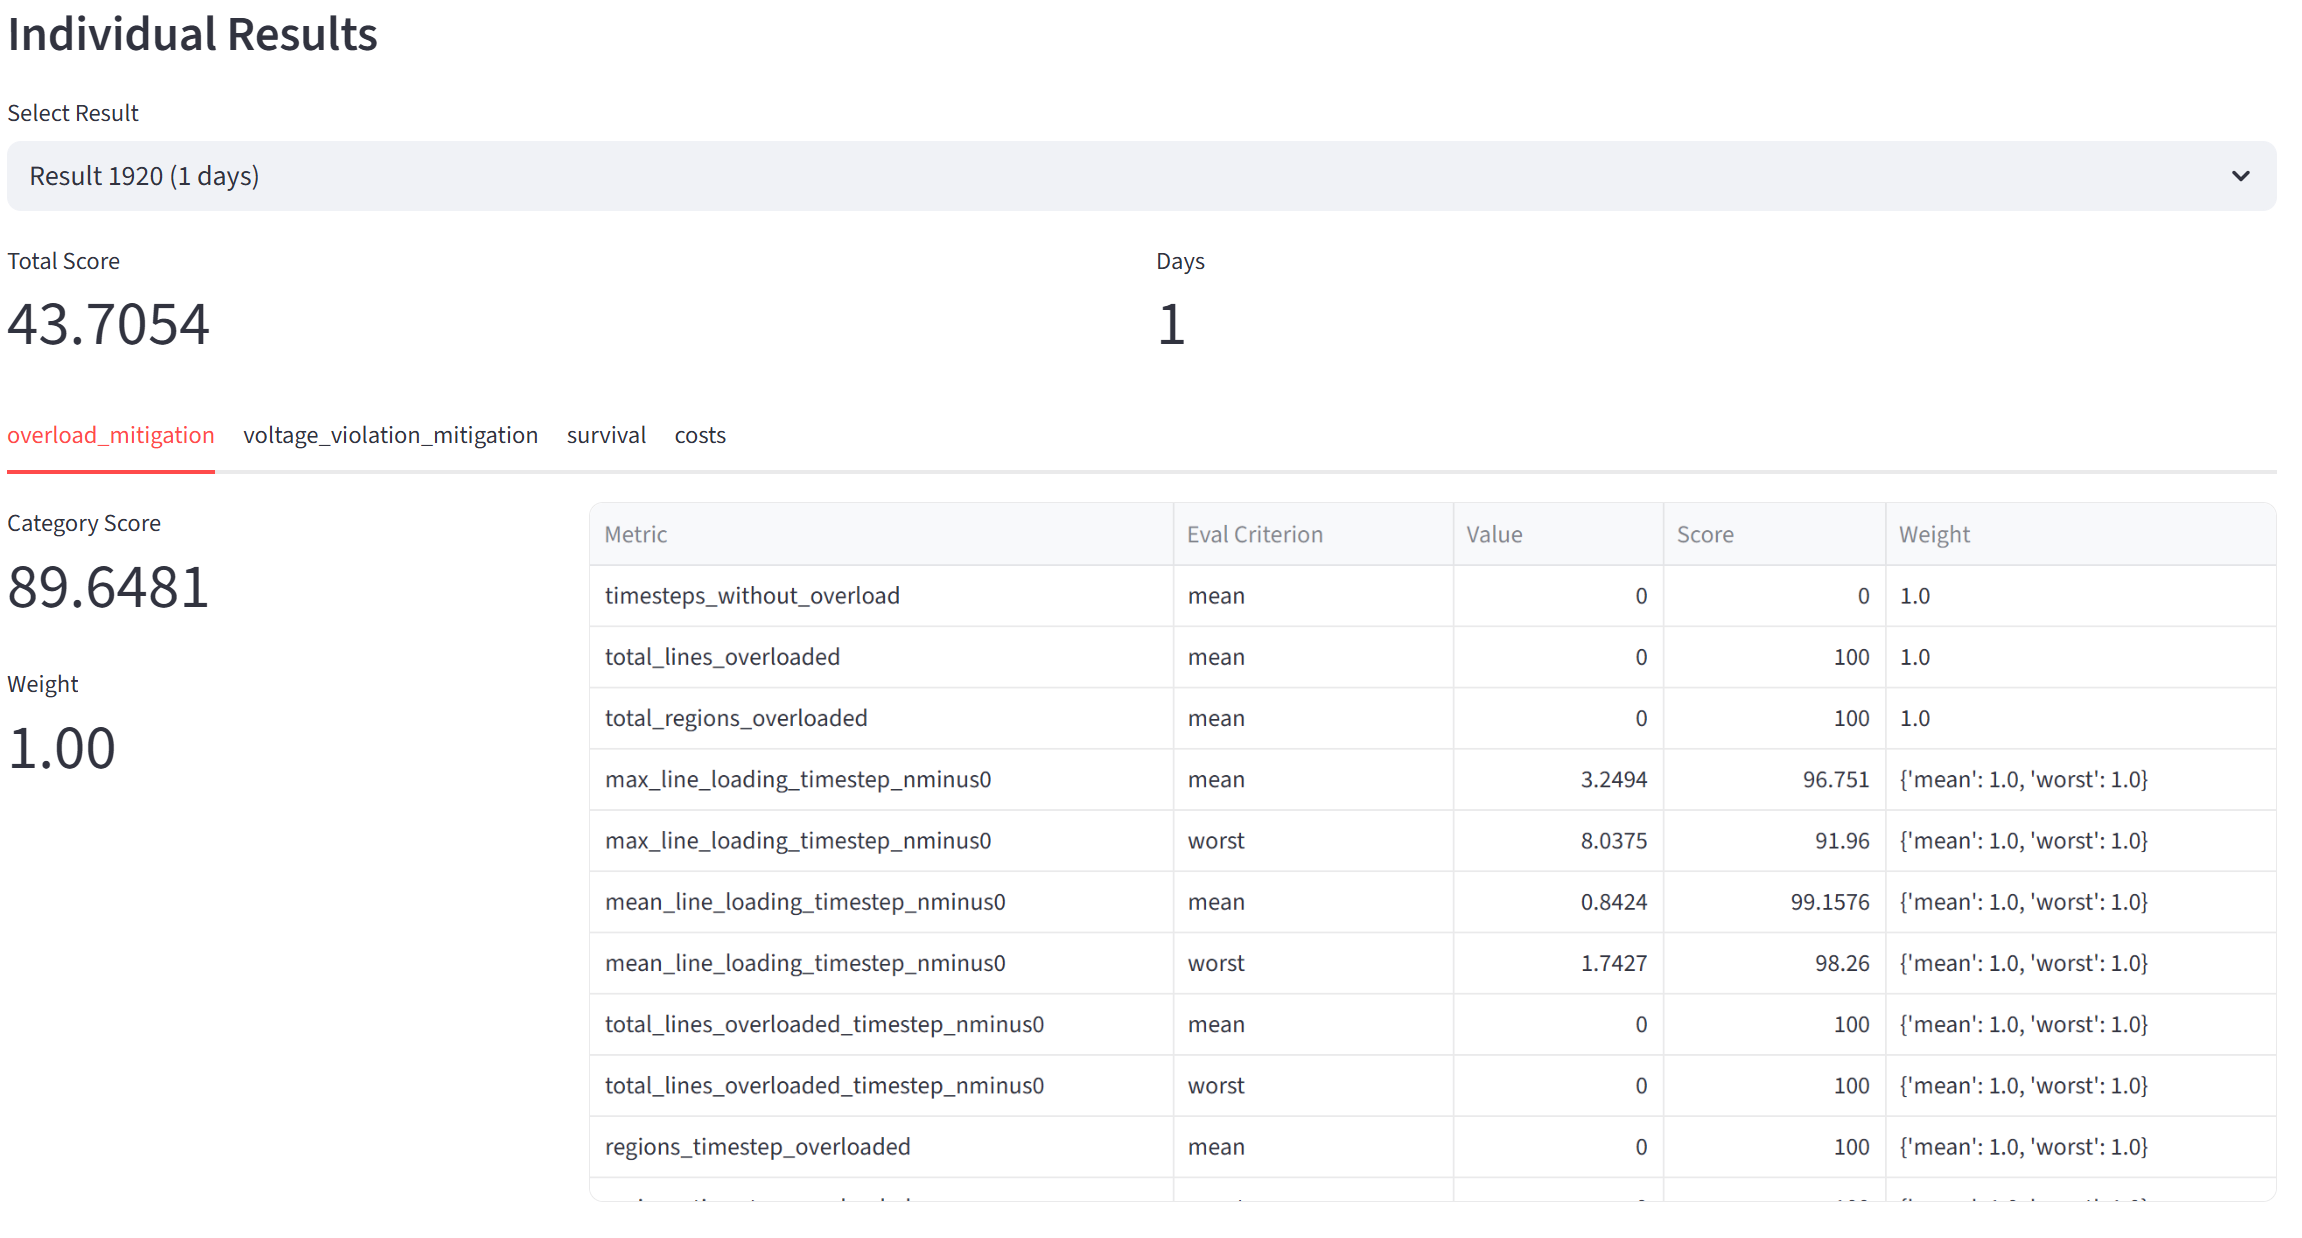
\includegraphics[width=\textwidth]{images/appendix/webapp/webapp_individual_results.png}
        \caption{Individual result section}
        \label{fig:webapp-individual-result}
    \end{subfigure}

    \caption{Overview over webapp sections (continued)}
\end{figure}


\FloatBarrier

\subsection{Summary Comparison Web Application}\label{app:comparison-webapp}
Figure \ref{fig:comparison-webapp-screenshots} shows screenshots of the Streamlit-based comparison web application, which is introduced in Section \ref{ssec:visual-feedback}.

\begin{figure}[htp]
    \centering
    \begin{subfigure}[t]{0.98\textwidth}
        \centering
        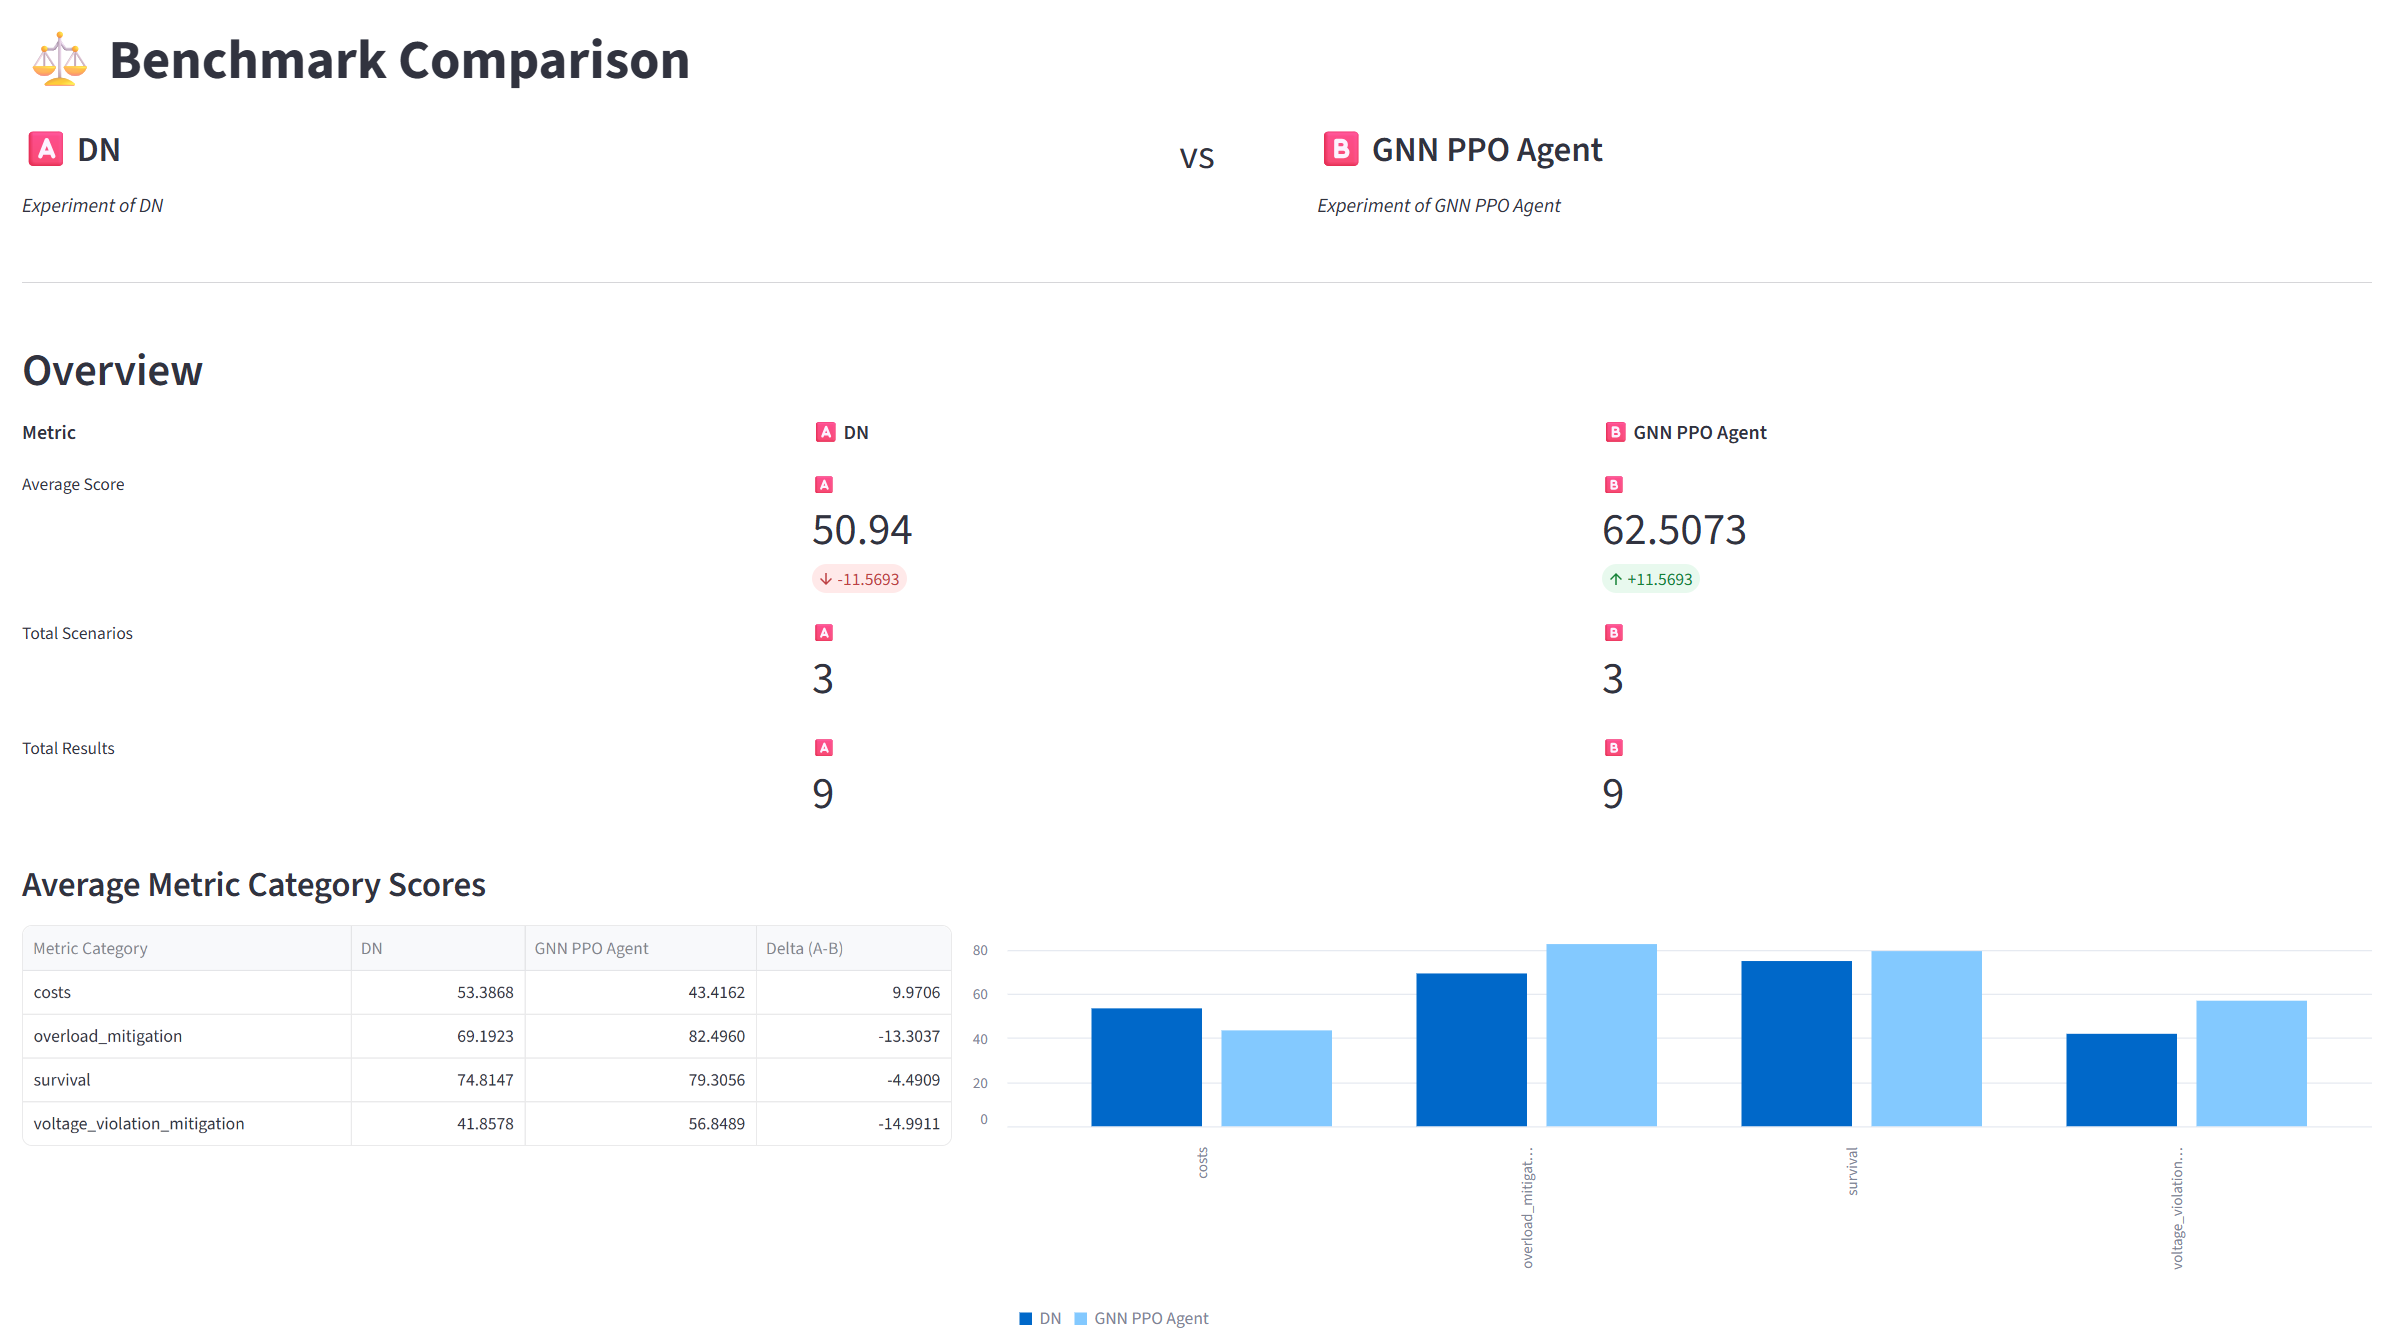
\includegraphics[width=\textwidth]{images/appendix/webapp/comparison_overview.png}
        \caption{Overview section}
        \label{fig:comparison-overview}
    \end{subfigure}

    \caption{Overview over comparison webapp sections, with do-nothing agent on the left, and a PPO agent on the right}
    \label{fig:comparison-webapp-screenshots}
\end{figure}

\begin{figure}[htp]
    \ContinuedFloat
    \centering

    \begin{subfigure}[t]{0.98\textwidth}
        \centering
        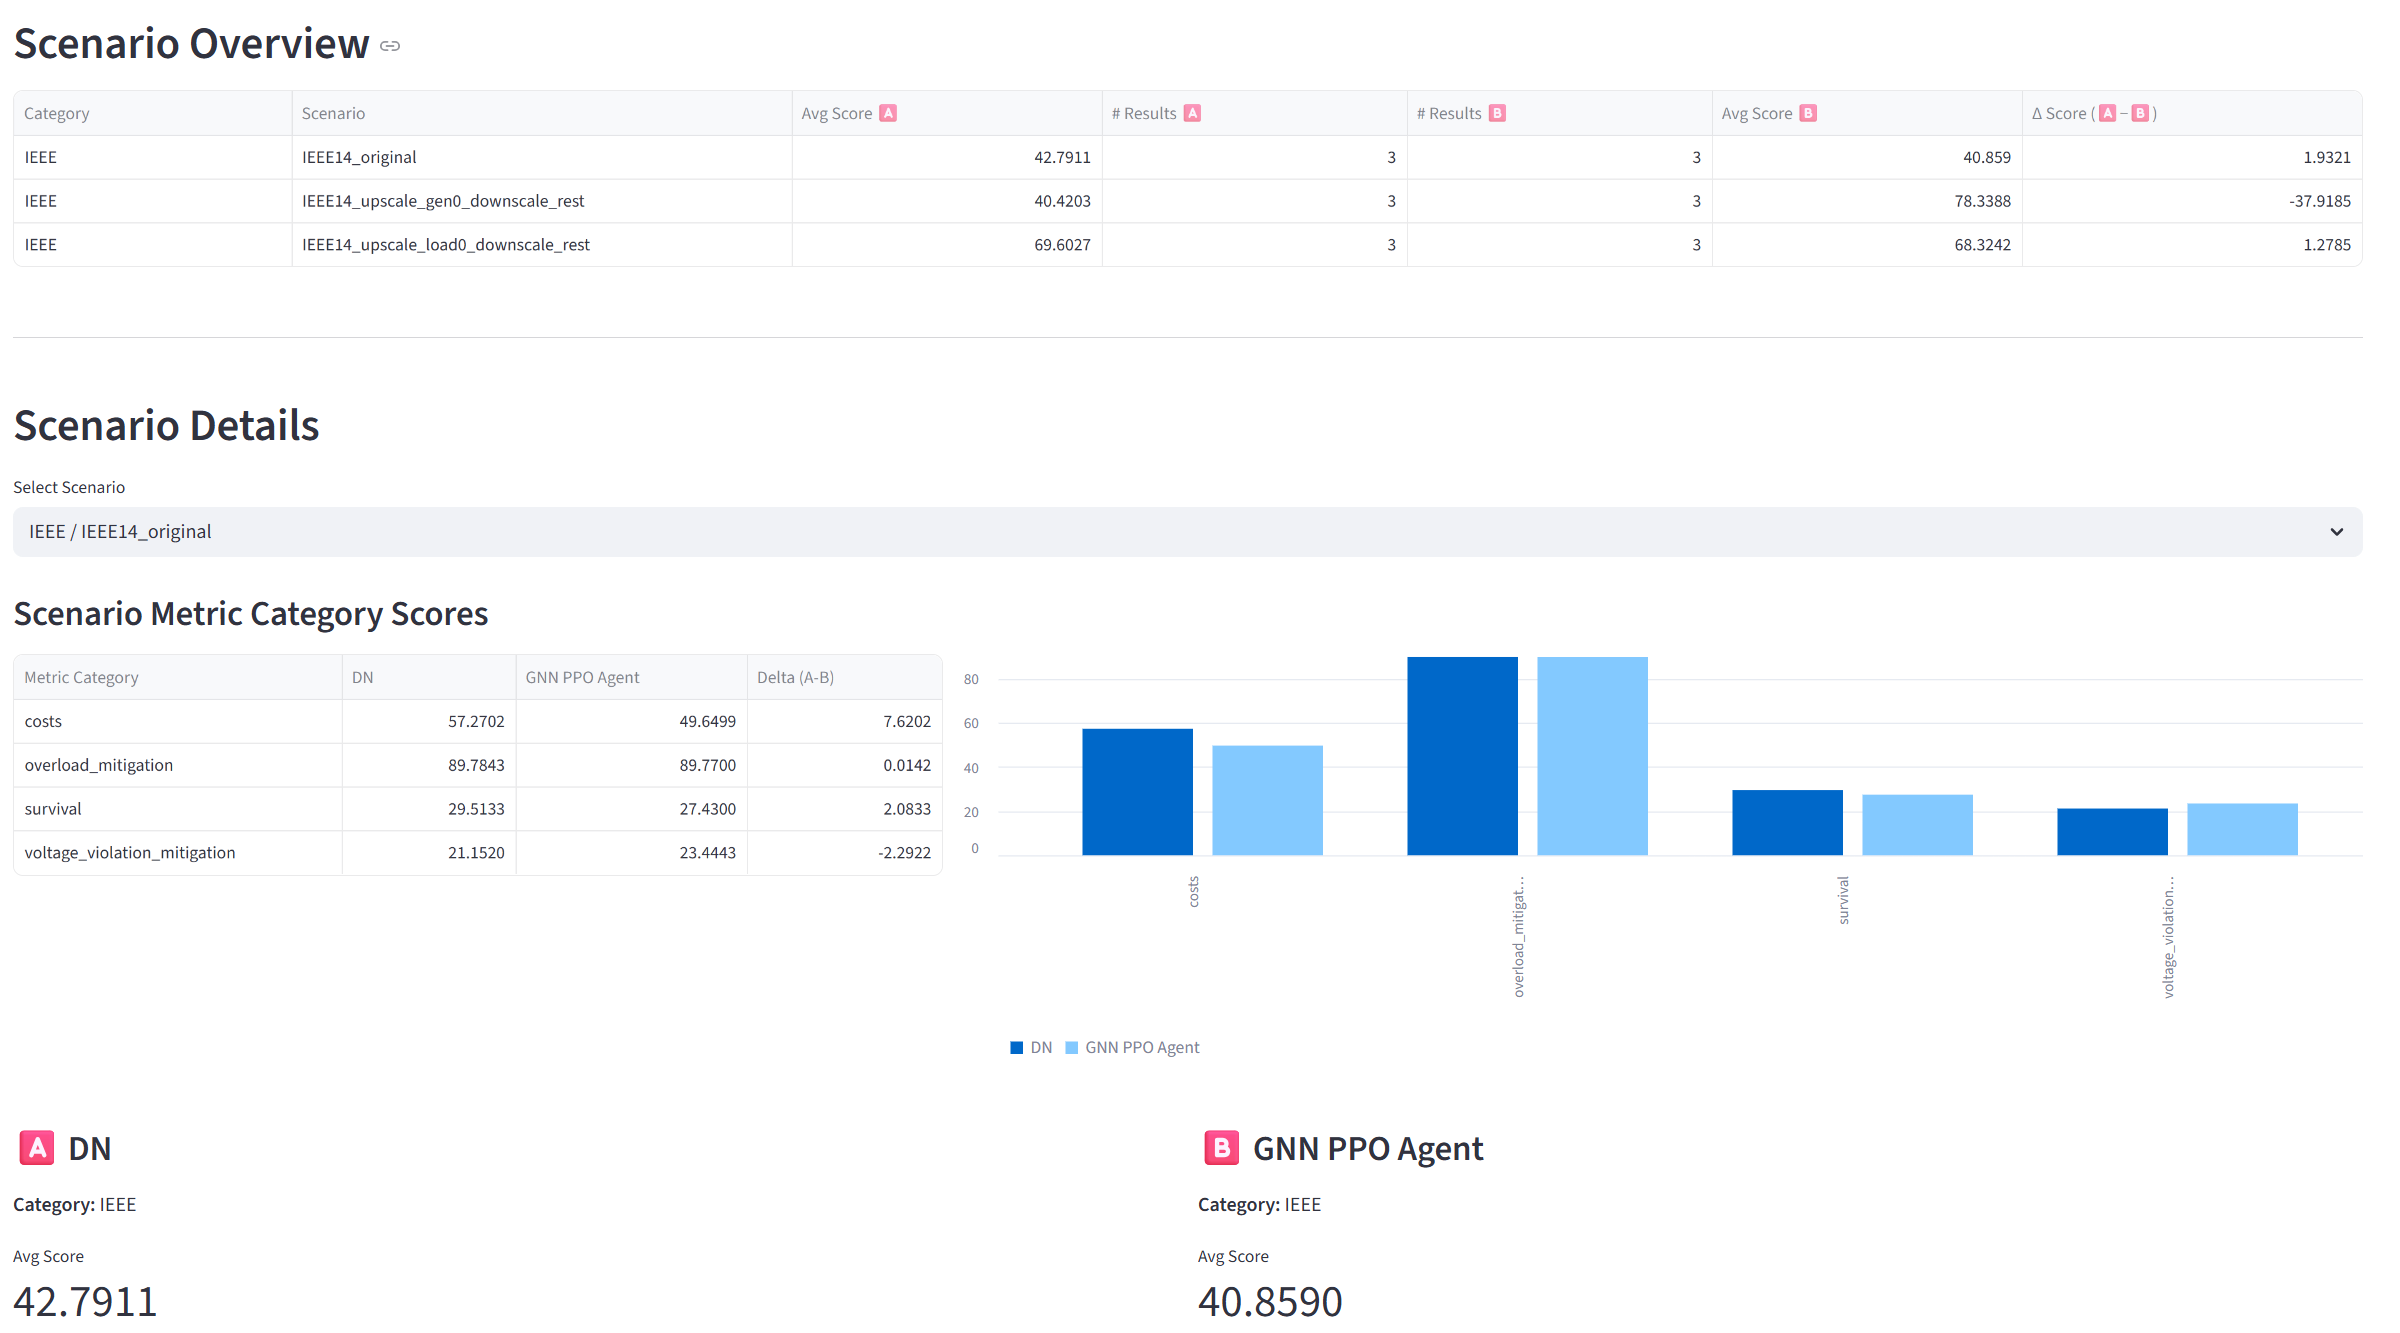
\includegraphics[width=\textwidth]{images/appendix/webapp/comparison_scenario_overview.png}
        \caption{Scenario overview section}
        \label{fig:comparison-scenario-overview}
    \end{subfigure}

    \vspace{0.1em}

    \begin{subfigure}[t]{0.98\textwidth}
        \centering
        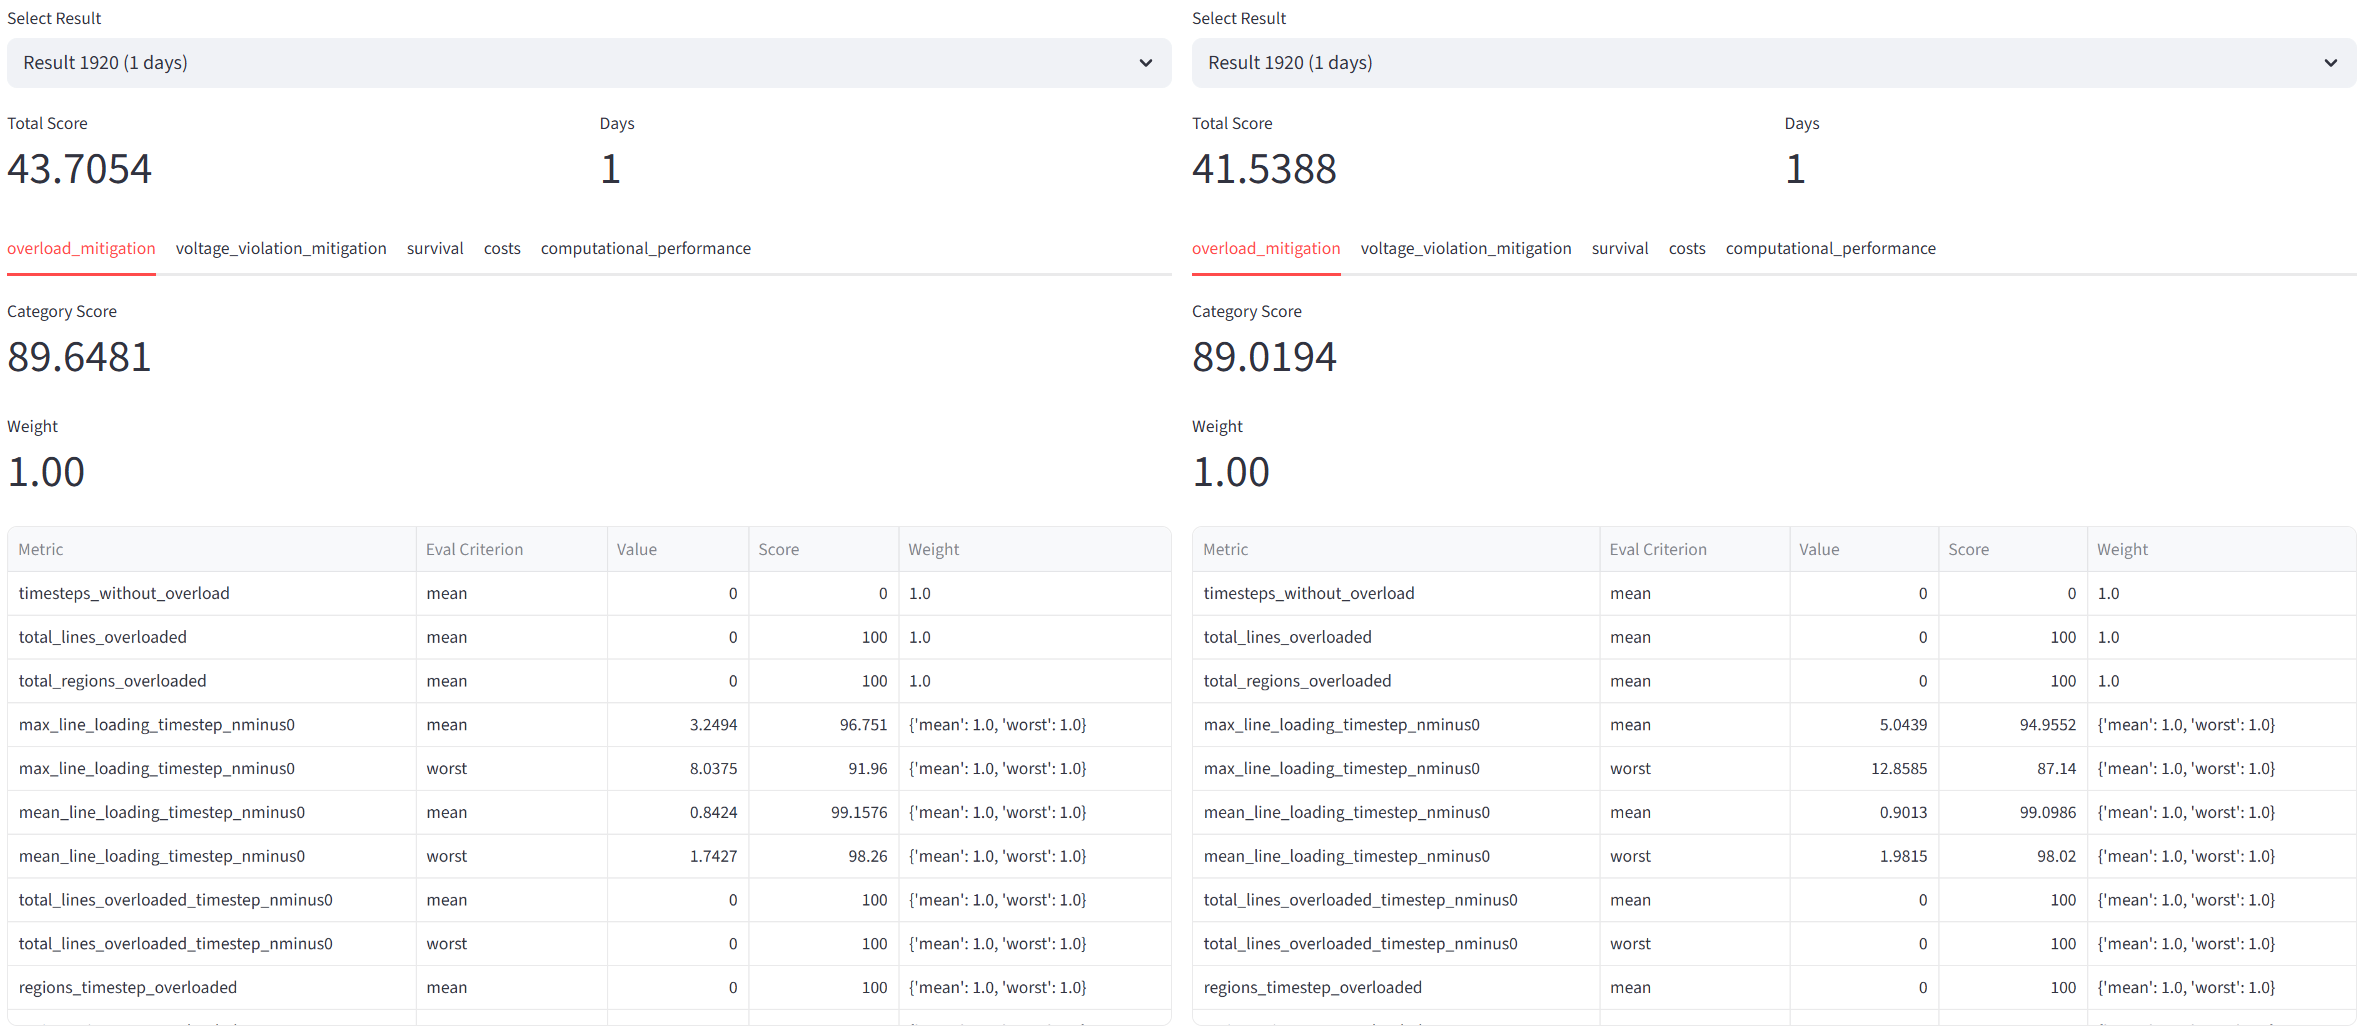
\includegraphics[width=\textwidth]{images/appendix/webapp/comparison_individual_results.png}
        \caption{Individual result section}
        \label{fig:comparison-individual-result}
    \end{subfigure}

    \caption{Overview over comparison webapp sections, with do-nothing agent on the left, and a PPO agent on the right (continued)}
\end{figure}

\FloatBarrier

\subsection{Replay Graphs}
Figure \ref{fig:replay-graphs} shows an example of the two graph views generated by the replay task described in Section \ref{ssec:replay-data}.

\begin{figure}[htp]
    \centering
    \begin{subfigure}[t]{0.9\textwidth}
        \centering
        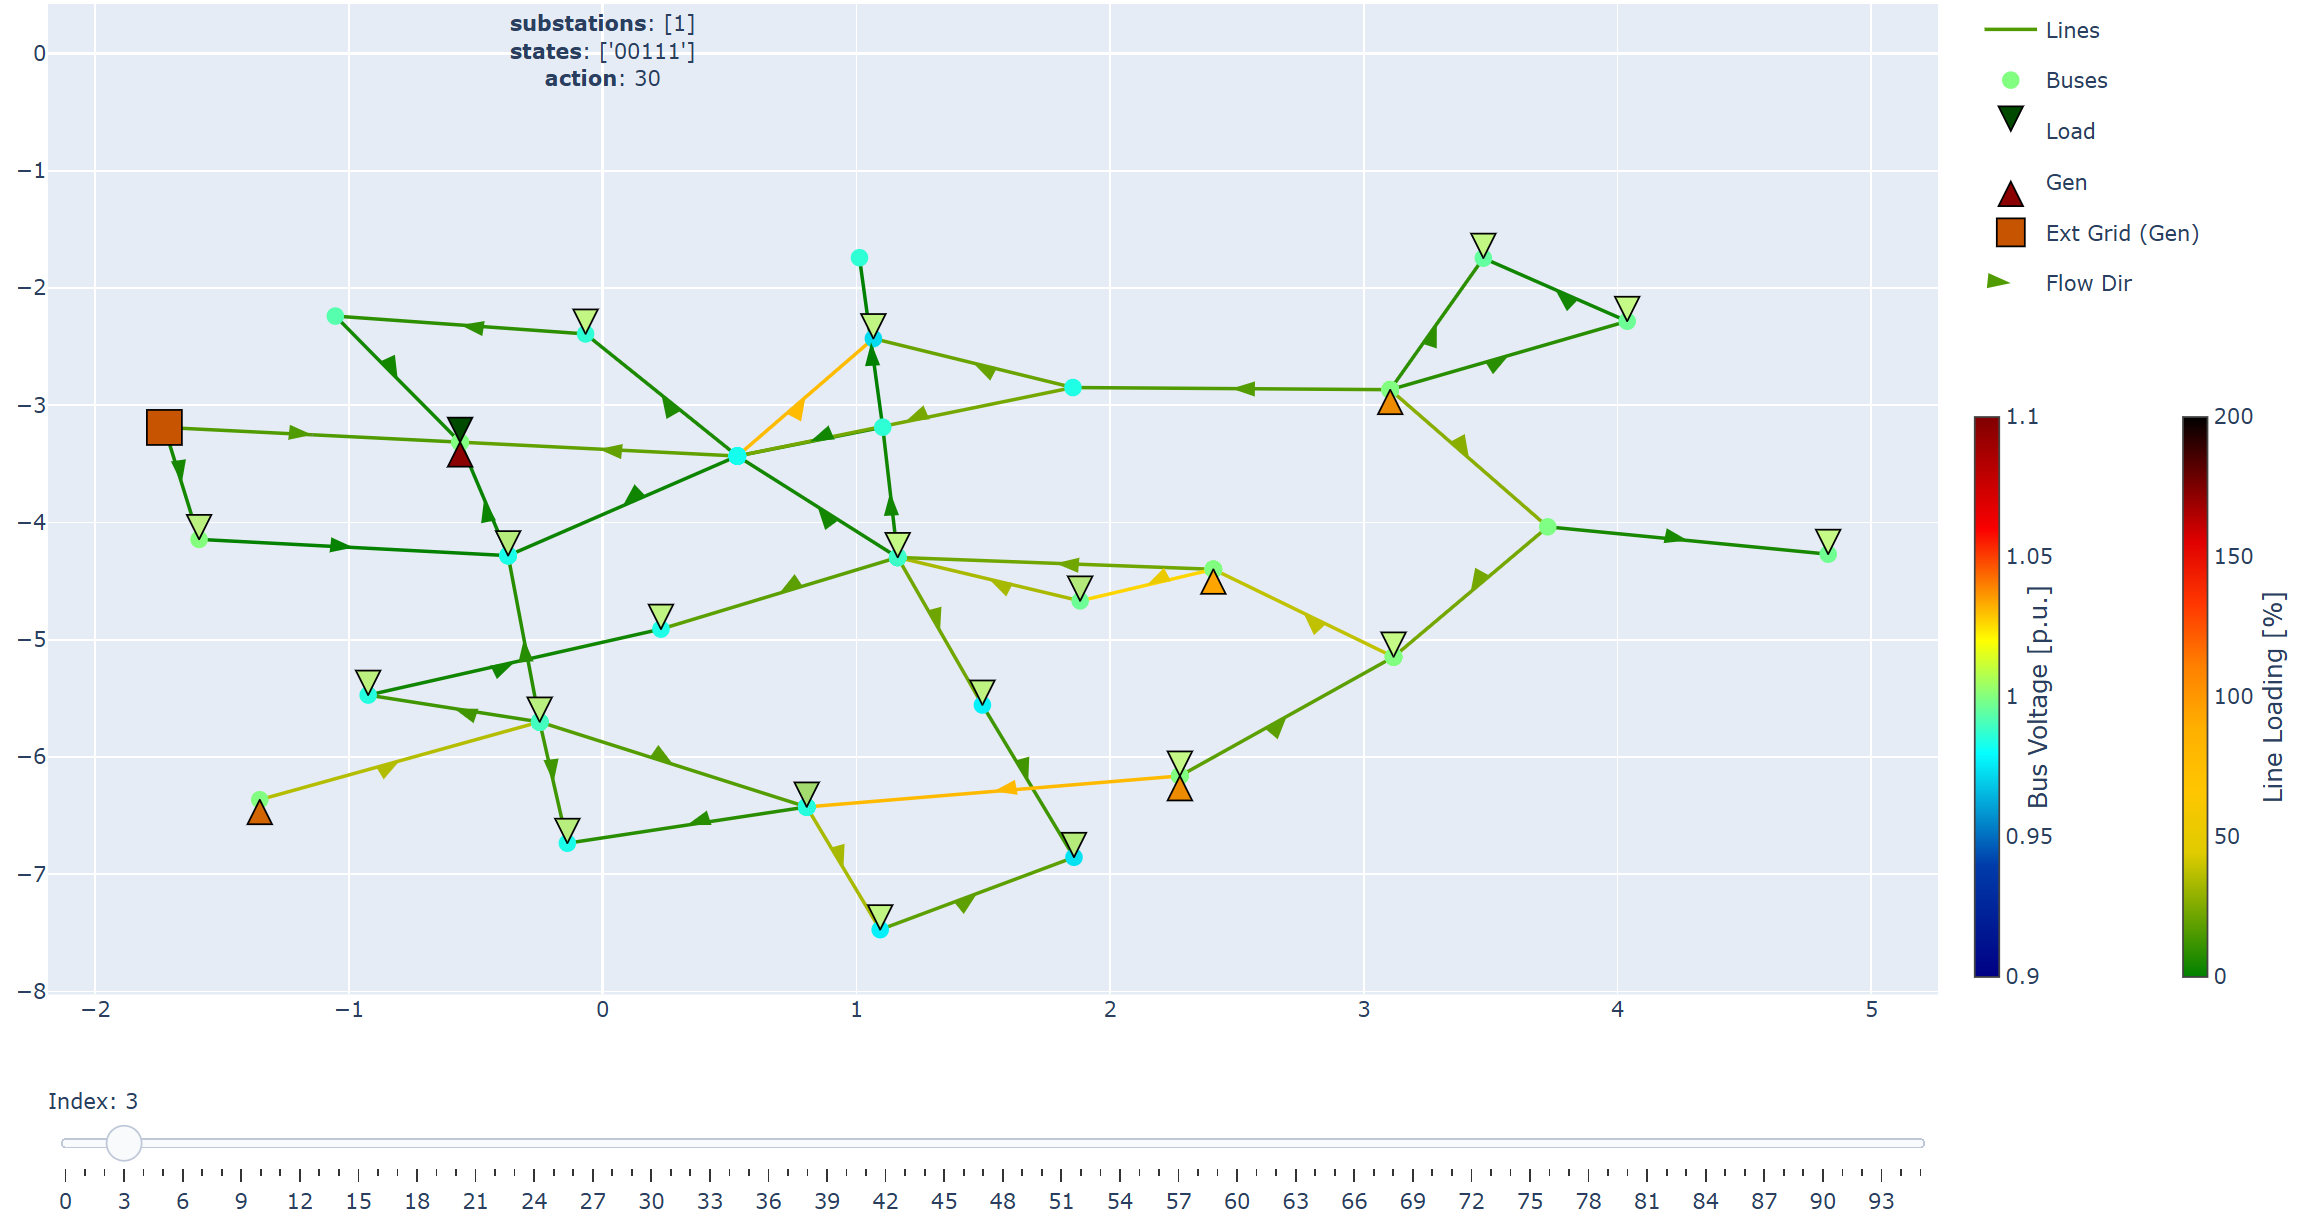
\includegraphics[width=\textwidth]{images/appendix/replay/network_graph.png}
        \caption{Network graph of the replay data, showing the limits of the grid}
        \label{fig:network-graph}
    \end{subfigure}

    \vspace{0.1em}

    \begin{subfigure}[t]{0.9\textwidth}
        \centering
        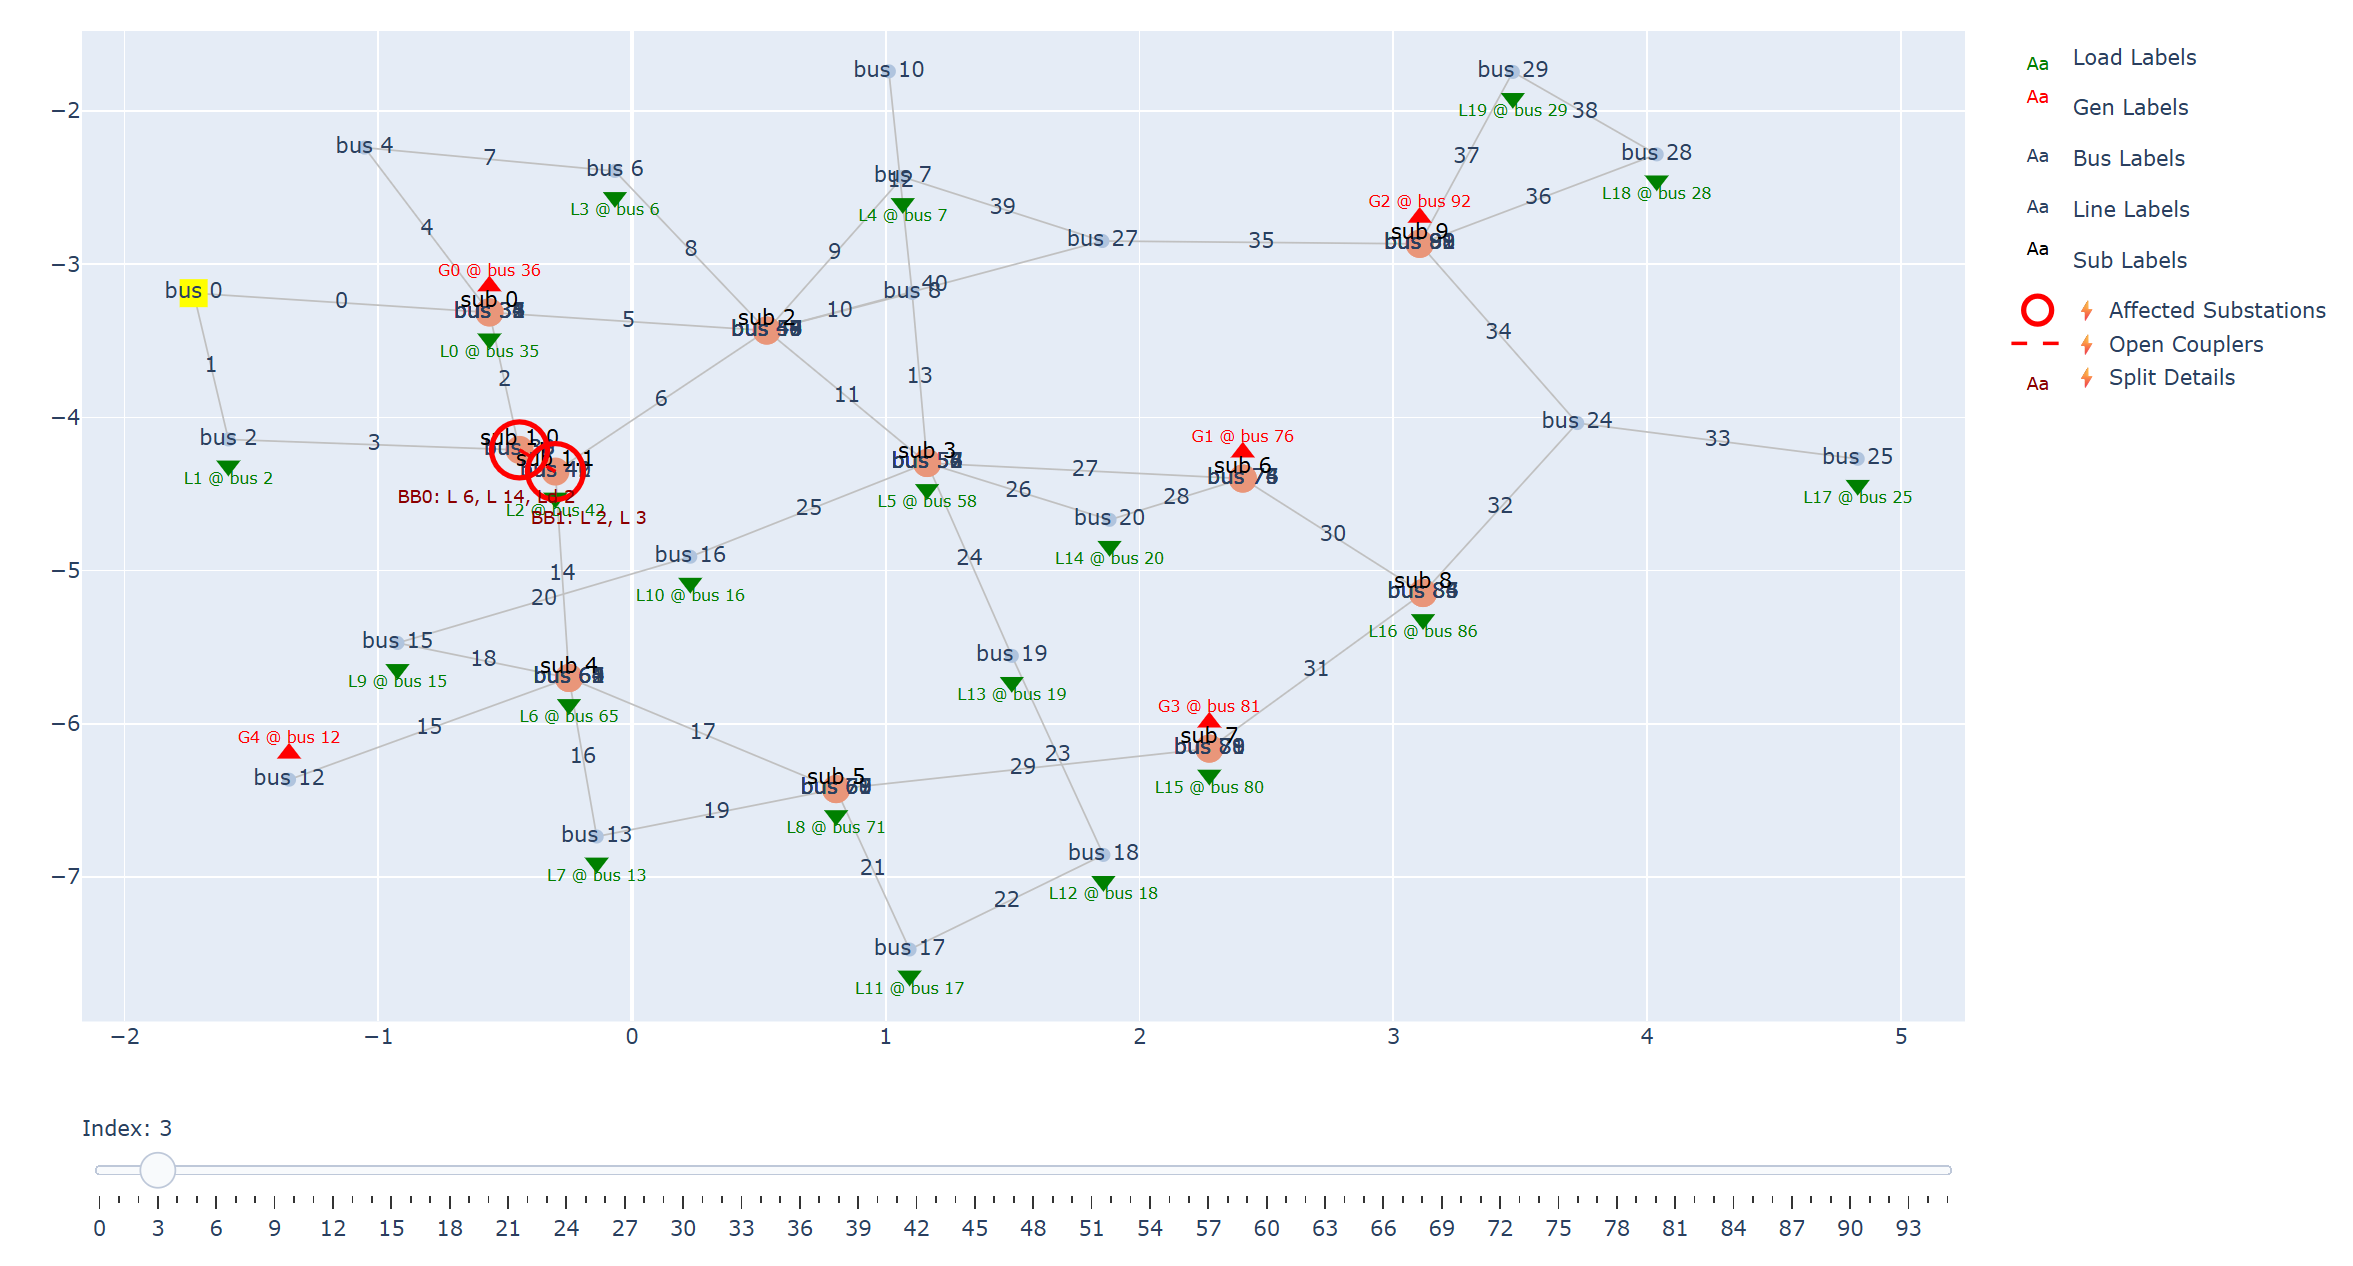
\includegraphics[width=\textwidth]{images/appendix/replay/action_graph.png}
        \caption{Action graph of the replay data, showing the actions of the agent}
        \label{fig:action-graph}
    \end{subfigure}

    \vspace{0.1em}

    \begin{subfigure}[t]{0.48\textwidth}
        \centering
        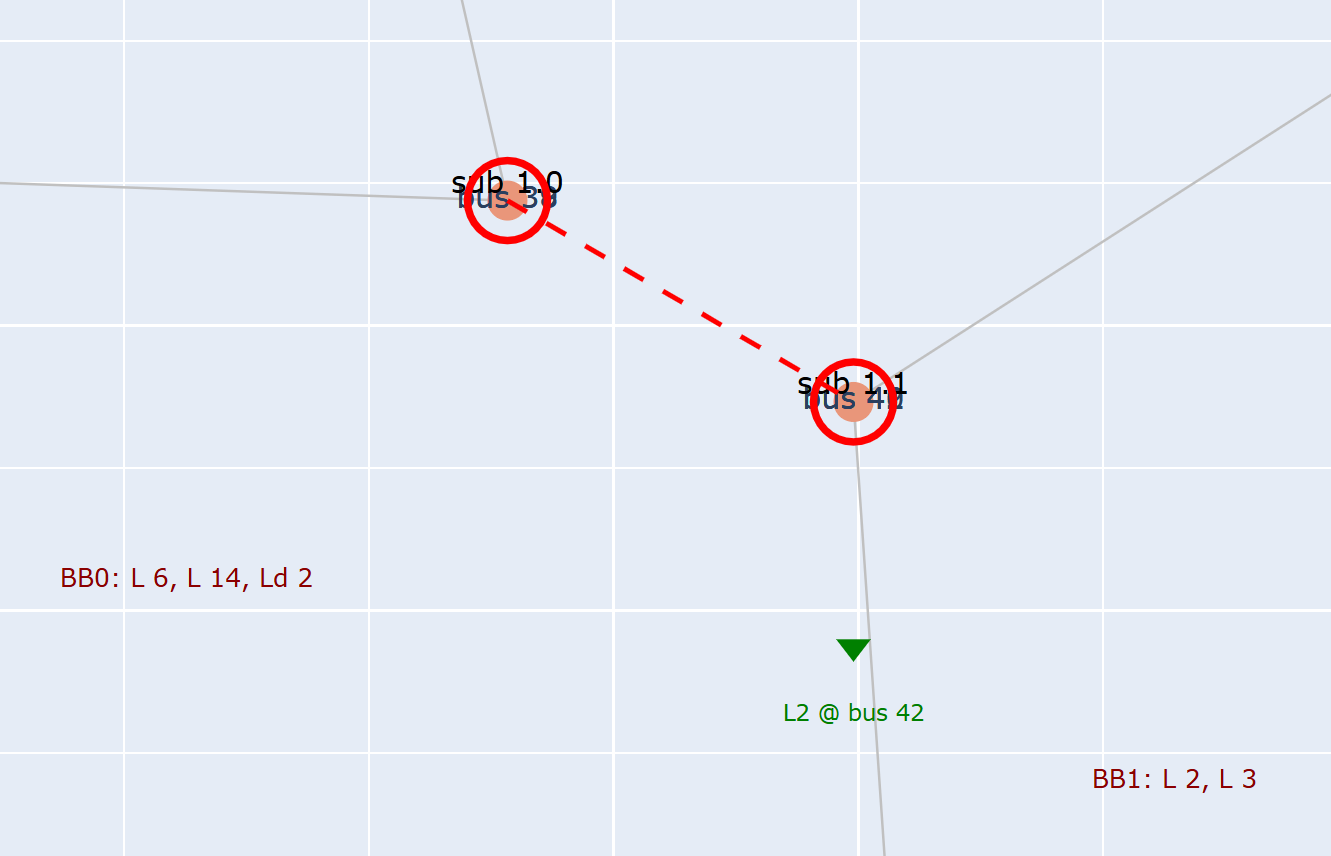
\includegraphics[width=\textwidth]{images/appendix/replay/action_graph_zoomed.png}
        \caption{Zoom-in of the action graph, showing bus-splitting}
        \label{fig:action-graph-zoomed}
    \end{subfigure}

    \caption{Overview over the replay data website, showing the two graph views}
    \label{fig:replay-graphs}
\end{figure}